\documentclass[11pt, twoside, letterpaper]{article}
\usepackage[utf8]{inputenc}
\usepackage[margin=0.6in]{geometry}
\usepackage{geometry}                   % See geometry.pdf to learn the layout options. There are lots.
\usepackage[parfill]{parskip}       % Activate to begin paragraphs with an empty line rather than an indent
\usepackage{graphicx}       % Use pdf, png, jpg, or eps§ with pdflatex; use eps in DVI mode
\usepackage{amssymb}
\usepackage{amsmath}
\usepackage{placeins}

\title{EE105 MiniProject: AM Radio}
\author{Michael Lin and Jene Li}
\date{December 2013}

\begin{document}

\maketitle

\section{Introduction}
\newpage

\section{Circuit Diagram}
\begin{figure}[htbp]
	\begin{center}
		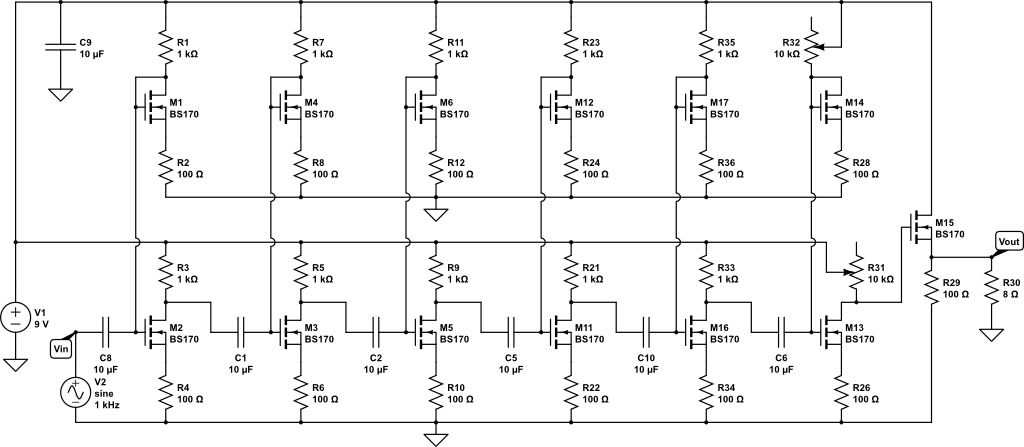
\includegraphics[scale=0.8,angle=-90]{circuitdiagram.png}
		\caption{Circuit Diagram}
	\end{center}
\end{figure}
\FloatBarrier
\newpage
\section{Topology}
We used a total of 6 stages in our amplifier. Five common sources and one source follower.
Our first decision was to choose topologies to use for amplification. We first considered using a cascode stage because of 
its characteristically high gain and good frequency response (high bandwidth). However, due to the high gain of the cascode
it was very difficult to bias it correctly such that it would not rail. The possible cascode configuration is shown in Figure 2,
We need to choose R1 and R2 carefully such that the current being forced by both PMOS and NMOS current mirrors are the same.
Otherwise, the small difference in current will reflect as a voltage drop in one of the $r_o$s and the high gain of the cascode
will amplify and rail this difference.
\begin{figure}[htbp]
\begin{center}
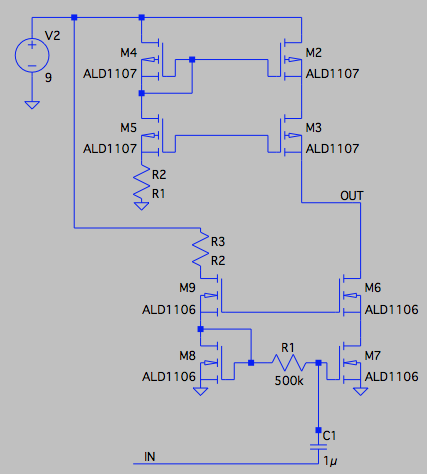
\includegraphics[width=4in,height=4in]{Cascode.png}
\caption{Cascode topology}
\end{center}
\end{figure}
\FloatBarrier

After some more consideration, we decided to use multiple stages of common source topologies as the one shown in Figure 3 because they would 
be much easier to bias than cascode stage. We also decided to use MOSFETS rather than BJTs because while they had lower gain than BJTs (the $g_m$ of MOSFETS
is in the order of $10^{-3}$ compared to the BJT's $0.038$), the large gate impedance of MOS proved more attractive since we dont have to
worry much about impedance loading between stages. As for the specific MOS, we used the BS170 N-channel MOSFETs because they had high saturation
current capacity and, thus, a higher $g_m$ and gain.

Going back to the biasing of the common sources. Our first decision was to choose a desired drain current so that the gain and the $V_{outBIAS}$
would depend on this current. We will go through this calculations in a later section, but it is easy to see that both drain current and 
$V_{outBIAS}$ are straight forward to bias. Drain current is set by using a current mirror, as shown in Figure 3. Then we choose our drain 
resistance such that we get a well centered $V_{outBIAS}$. In our case, we chose $R_D=1000k\Omega$, so the voltage drop on the resistor would be 
6V and leave a $V_{outBIAS}\approx 4V$. The gain per common source stage turned out to be low and inconsistent across different BS170, probably
due to their mismatch in $\frac{W}{L}$, in fact, it was a gain ranging from 5 to 10. However, since we did not have inter-stage loading gain loss,
cascading multiple of this common sources would increase our gain exponentially with a base in the range of 5 to 10. So five stages were enough
to reach a gain of over 12500.

Between each of the common source stages we AC couple with a 10uF capacitor and individually bias each stage with its own current mirror circuit
as shown in Figure 1.

\begin{figure}[htbp]
\begin{center}
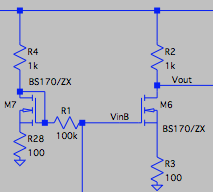
\includegraphics[width=3in,height=3in]{CurrentMirror.png}
\caption{Current Mirror Biasing a Common Source}
\end{center}
\end{figure}
\FloatBarrier

The last stage of our amplifier is a Common Drain. We decided to use a common drain for multiple reasons. The first one and the main one
is that its output resistance is very small, approximately $\frac{1}{g_m}$. As we mentioned earlier our current of 6mA gives us a $g_m\approx10^{-3}s$
so the impedance looking into the source of the MOSFET is $\approx 1000\Omega$. Even though the gain of our source follower is approximately unity we
still have some gain loss since the load we are trying to drive is $8\Omega$ and the voltage division will attenuate the signal by 100=40dB however 
since the gain from our amplifier is high enough that our final circuit gain is around 82dB which we will show later in the simulation and calculations. 
To drive our $8\Omega$ speaker with $1V_{pp}$ we use a $100\Omega$ resistor in parallel to draw some of the current and not burn the speaker with 
1000/8=125mA. Another reason we use a source follower is that it has a good current gain, technically it has infinite current gain since there is no
current going into the gate but the current throughput is enough to get it up to around 40mA to drive the speaker. We can see the implementation of the
loading stage (source follower and speaker load) in Figure 4. To get a current as high as 40mA we had to bias the gate with a high enough voltage, so
since the $V_{outBIAS}$ of the previous common source stage was already biased to around 4V, we decided to DC couple this last loading stage using 
the bias from the output of the last stage of common source as we can see in Figure 1.

\begin{figure}[htbp]
\begin{center}
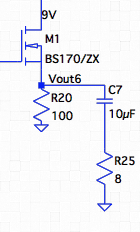
\includegraphics[width=2in,height=3in]{SourceFollower.png}
\caption{Source Follower: Loading Stage}
\end{center}
\end{figure}
\FloatBarrier

At last we implemented volume control using a potentiometer 

\section{Hand Calculations and Measurements}
\subsection*{Magnitude/Phase Bode Plot}
\begin{figure}[htbp]
\begin{center}
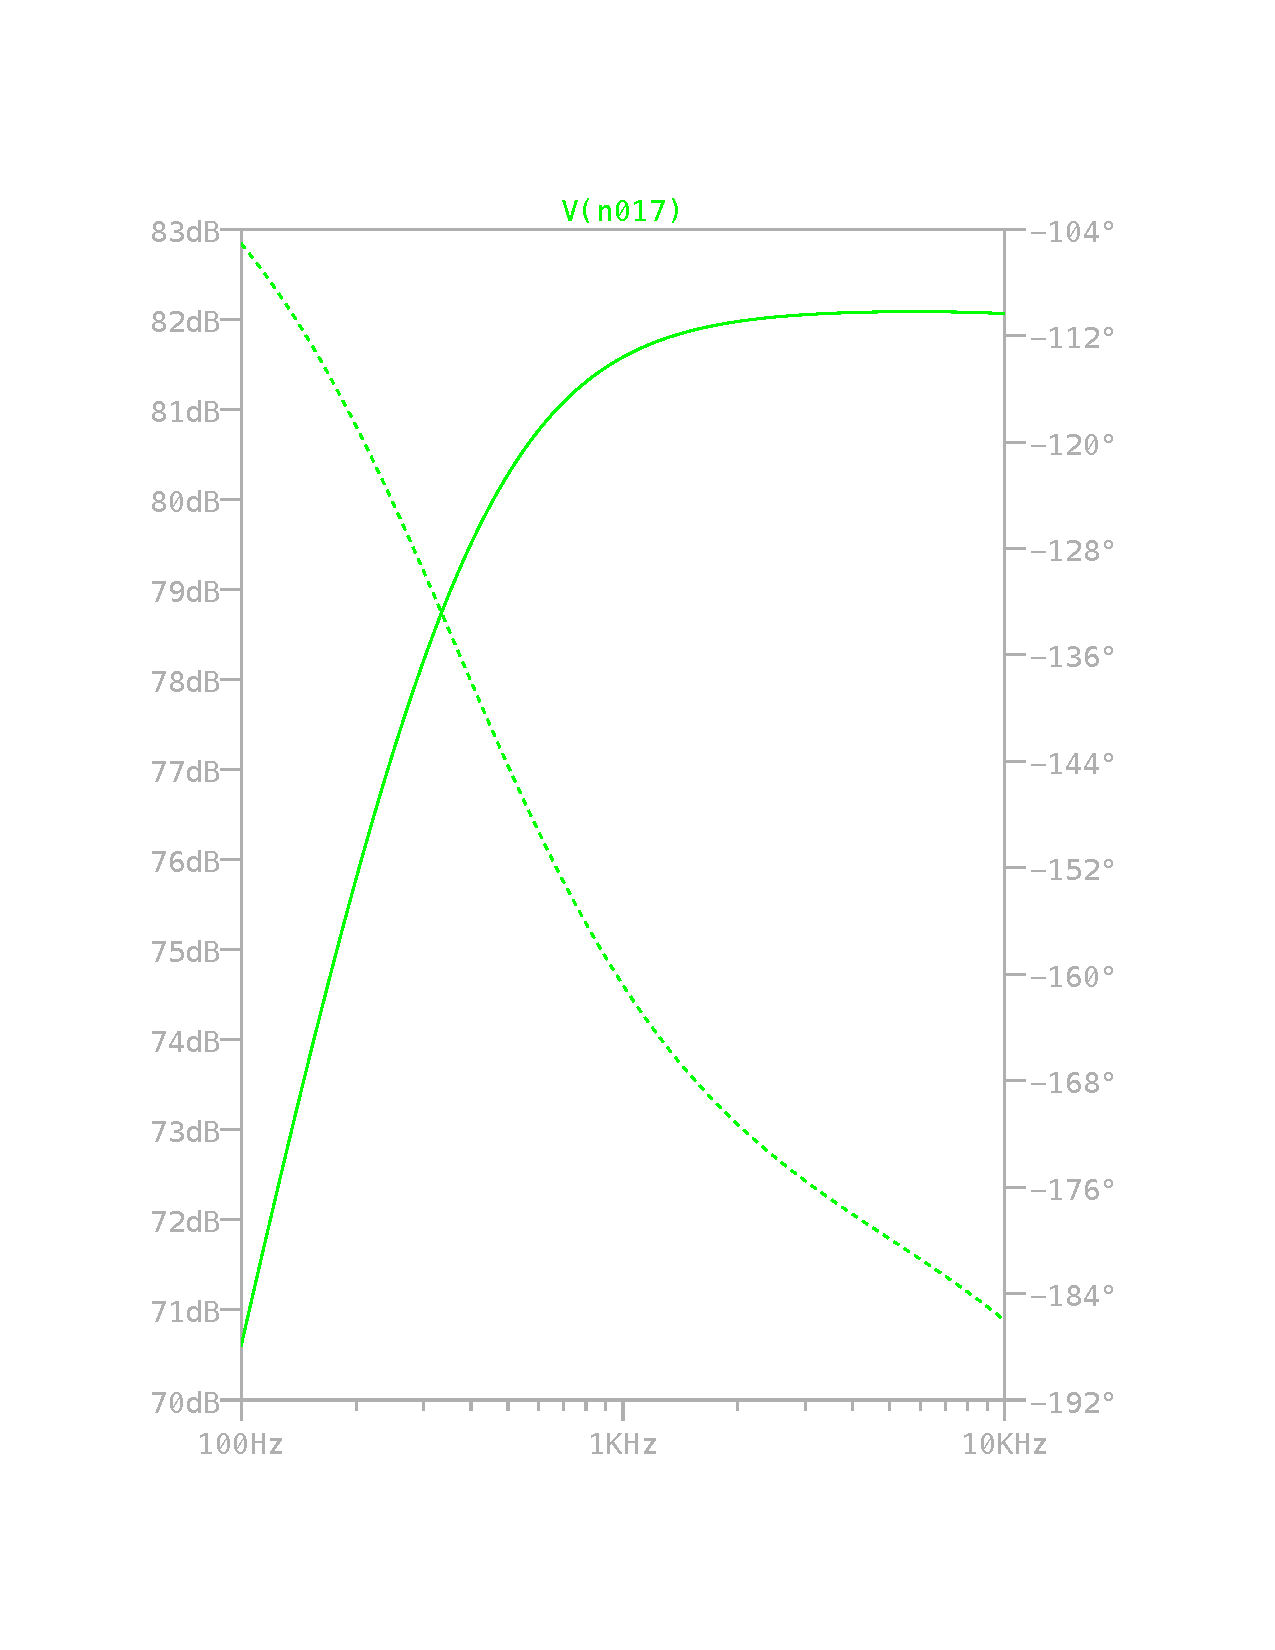
\includegraphics[width=4in]{MagPlot.pdf}
\caption{Current Mirror Biasing a common source}
\end{center}
\end{figure}
\FloatBarrier

\subsection*{Output Impedance}
\subsection*{Bias Voltages/Currents}
\begin{tabular}{|r|l|l|}
\hline
Stage & $V_{GS}$ & Drain Current\\
\hline
Stage 1 &2.32V&6.33mA\\
Stage 2 &2.4V&6.2mA\\
Stage 3 &2.37V&5.14mA\\
Stage 4 &2.48V&4.55mA\\
Stage 5 &4.7V&41mA\\
Stage 6 &2.8V&35mA\\
\hline
\end{tabular}
\subsection*{Power Consumption}

\end{document}
